\documentclass[a4paper, 10pt]{article}
\usepackage[margin = 1in]{geometry}
\usepackage{amsmath}
\usepackage{tabularx}
\usepackage{framed}
\setlength{\parindent}{0em}
\newcolumntype{L}{>{\arraybackslash}m{4cm}}
\newcolumntype{T}{>{\arraybackslash}m{6cm}}
\usepackage{graphicx}
\usepackage{pdfpages}

\begin{document}

\section*{Topic 9 - First Law of Thermodynamics}

\section{Specific heat capacity and specific latent heat}
\subsection{Heat capacity}
\begin{frame}
The numerical value of the heat capacity of a body is the quanttity of heat required to raise the temperature of the body by one degree
\[
C = \frac{Q}{\Delta T}
\]
\end{frame}	
\subsection{Specific heat capacity}
\begin{framed}
   the numerical value of the specific heat capacity of a substance is the quantity of heat required to raise the temperature of the unit mass of the substance by one degree
   \[
   c = \frac{Q}{m\Delta T}
   \]
\end{framed}	

\subsection{Determination of specific heat capacity}
\textbf{For solids}, since
\[
  IVt = mc(T_f - T_i)
\]

\[
   c = \frac{IVt}{m(T_f - T_i)}
\]

\textbf{For gases or liquids}, to account for heat loss
\begin{center}
   electrical energy supplied = heat transferred to liquid + HEAT LOSS to surrounding
\end{center}	

\[
   IV \times t = mc(T_{out} - T_{in}) + H
\]

\[
   IV = \frac{m}{t}c (T_{out} - T_{in}) + \frac{H}{t}
\]

rate of heat loss $\frac{H}{t}$ is proportional to the excess temperature of the apparatus. \\

using a different set of $I, V$ and flow rate, 
\[
   I'V' = \frac{m'}{t'}c (T_{out} - T_{in}) + \frac{H'}{t'}
\]

using the two sets of equations, 
\[
   IV - I'V' = \left( \frac{m}{t} - \frac{m'}{t'} \right) (T_{out} - T_{in})\  c
\]

\subsection{Kinetic model of matter} 
\begin{center}
   \begin{tabular}{L | L | L | L}
      & solid & liquid & gas \\
      \hline
      packing arrangement of atoms/molecules & closely packed in lattice structure 
                                             & slightly further apart than solids & 
                                             very far apart \\ 
                                             \hline
      movement of atoms & vibrations about mean position & random motion throughout liquid & random motion at high speeds \\ 
      \hline
      intermolecular forces & strong intermolecular attractive and repulsive forces & attractive forces & negligible intermolecular forces 
   \end{tabular}
\end{center}

\subsection{Change of phase}
\begin{center}
   \begin{tabular}{L | T | T}
      & Melting & Boiling \\
      \hline 
      intermolecular interactions & lattice structure starts to break & all bonds between atoms/molecules completely broken \\
      & 
      \begin{itemize}
         \item molecules have enough energy to vibrate so violently that they are no longer held by attractive forces
         \item the lattice structure collapses
         \item change of state occurs
      \end{itemize}	
      & 
      \begin{itemize}
         \item thermal energy supplied is used to overcome the attractive forces between molecules
         \item bonds are completely broken
         \item change of state occurs
      \end{itemize}	
      \\
      energy supplied & latent heat of fusion & latent head of vaporisation \\
      \hline
   \end{tabular}
\end{center}

\textbf{standard qualitative questions}
\begin{enumerate}
   \item Why do melting and boiling take place without a change in temperature?
      \begin{itemize}
         \item at melting: lattice structure collapses due to vibration of molecules and solid uner goes phase change
         \item latent heat of fusion will not cause a change in temperature, and is used to overcome the attractive forces between atoms and causes the lattice structure to break
         \item during boiling: intermolecular forces are completely broken
         \item latent heat of evaporation used to overcome attractive forces between molecules
      \end{itemize}	
   \item Why is specific latent heat of vaporisation higher than the specific latent heat of fusion for the same substance?
      \begin{itemize}
         \item To melt a solid, some molecular bonds are broken
         \item to vaporise a liquid, all remaining bonds must be broken
         \item more bonds broken during vaporisation
         \item furthermore, work is needed to do work against the external or atmospheric pressure for gas to expand, since gas occupies a much larger volume than liquid
      \end{itemize}	
   \item Why is evaporation accompanied by cooling? 
      \begin{itemize}
         \item Kinetic theory supposes that molecules of liquids are at continual random motion and make frequent collisions with each other. During collision, some lose energy and some gain energy
         \item if a molecule near the surface gains enough evergy, it will be able to escape from the attractive forces from the molecules below it
         \item this results in a decrease in the average KE of the remaining molecule
         \item since temperature is a measure of average KE, the liquid becomes coller
      \end{itemize}	
\end{enumerate}	

\subsection{Latent heat}
\begin{framed}
   The numerical value of the specific latent heat of fusion is the quantity of heat required to convert unit mass of solid to liquid without any change in temperature

   \[
   l_f = \frac{Q}{m}
   \]

   The numerical value of specific latent heat of fusion is the quantity of ehat required to convert unit masss of liquid to gas without any change in temperature 
   \[
   l_v = \frac{Q}{m}
   \]
\end{framed}	

\subsection{Determination of latent heat}
For latent heat of fusion, to account for melting due to heat gained from surrounding
\begin{center}
   heat from electrical heater + heat gained from surrounding = latent heant of fusion 
\end{center}	
Let $M$  be the total mass of ice melted and $m$ be the mass of ice melted due to surroundings
\[
IV t + ml_f = Ml_f
\]
\[
   IV t = (M-m) l_f
\]
\[
l_f = \frac{IVt}{M-m}
\]

For latent heat of vaporisation, to account for heat loss to the surrounding
\[
IV = \frac{m}{t}l_v + \frac{H}{t}
\]
\[
I'V' = \frac{m'}{t'}l_v + \frac{H'}{t'}
\]

\[
l_v = \frac{IV - I'V'}{\frac{m}{t} - \frac{m'}{t'}}
\]

\section{Internal energy}
\begin{framed}
   The internal energy of a system is determined by the state of the system and it is the sum of the random distribution of kinetic and potential energies associated with the molecules of the system \\
   The internal energy of a system is the sum of KE due to \textbf{random motion} of the molecules, and PE associated with the \textbf{intermolecular forces of the system}
\end{framed}	

\textbf{Microscopic KE}
\[
   \angle E_k \rangle = \frac{3}{2}kT
\]

\textbf{Microscopic PE} \\
Molecules have PE due to intermolecular attraction and repulsion. Solids have the most negative PE

\textbf{Effect of temperature}
A rise in temperature implies an increase in average KE, hence an increase in internal energy

\subsection{Internal energy of an ideal gas}
Since it is assumed that an ideal gas has \textbf{no intermolecular forces}, the internal energy of a gas is purely due to translational KE \\

for one molecule
\[
   \langle E_k \rangle = \frac{1}{1}m\langle c^2 \rangle = \frac{3}{2}kT
\]

For N molecules
\[
   \text{total } E_k = \frac{1}{2}Nm\langle c^2 \rangle  = \frac{3}{2}NkT
\]

Since the internal energy $U$ of an ideal gas is purely kinetic
\[
   U = \text{total } E_k - \frac{3}{2}NkT
\]

\[
U = \frac{3}{2}NkT = \frac{3}{2}nRT = \frac{3}{2}pV 
\]
The \textbf{state} of a system is purely determined by $p$, $V$ and $T$ 
\begin{itemize}
   \item $\Delta U$ is solely dependent on T
   \item only a change in $p$ or $V$  which results in a change in $T$ will cause a change in state
\end{itemize}	

\section{First law of thermodynamics}
\begin{framed}
   the \textbf{First law of thermodynamics} states that the increase in internal energy of a system is equal to the sum of the heat supplied to the system and the work done on the system, and the internal energy of a system depends only on its state

   \[
   \Delta U = Q + W
   \]
\end{framed}	

\begin{center}
   \begin{tabular}{c | c | c}
      & Positive (+) & Negative (-) \\
      \hline
      $\Delta U$ & increase in internal energy & decrease in internal energy  \\
      $Q$ & Heat absorbed by the system & Heat loss by the system \\ 
      $W$ & Work done on system (compression) & Work done by system (expansion) \\
   \end{tabular}
\end{center}

\subsection{Work done, W}
for a gas in an enclosed system with a frictionless, movable piston of area A, when gas expands, a force $F$ is applied on the piston \textbf{by} the gas against external pressure $p$  \\

work done on the gas is thus 
\[
   W = - \int_{V_i} ^{V_f} pdV
\]

An increase in volume means work done on gas is negative

\subsection{pressure-volume graphs}
\begin{itemize}
   \item Internal energy U is dependent on state and change in internal energy
   \item $\Delta U$ is independent of path taken
   \item Work done $W$ is path dependent, and is the area under the P-V curve
\end{itemize}	


\subsection{Isobaric process}
Volume changes at constant pressure. Area under curve is rectangular and magnitude of work done is $p\Delta V$ \\
\begin{minipage}{0.5\textwidth}
      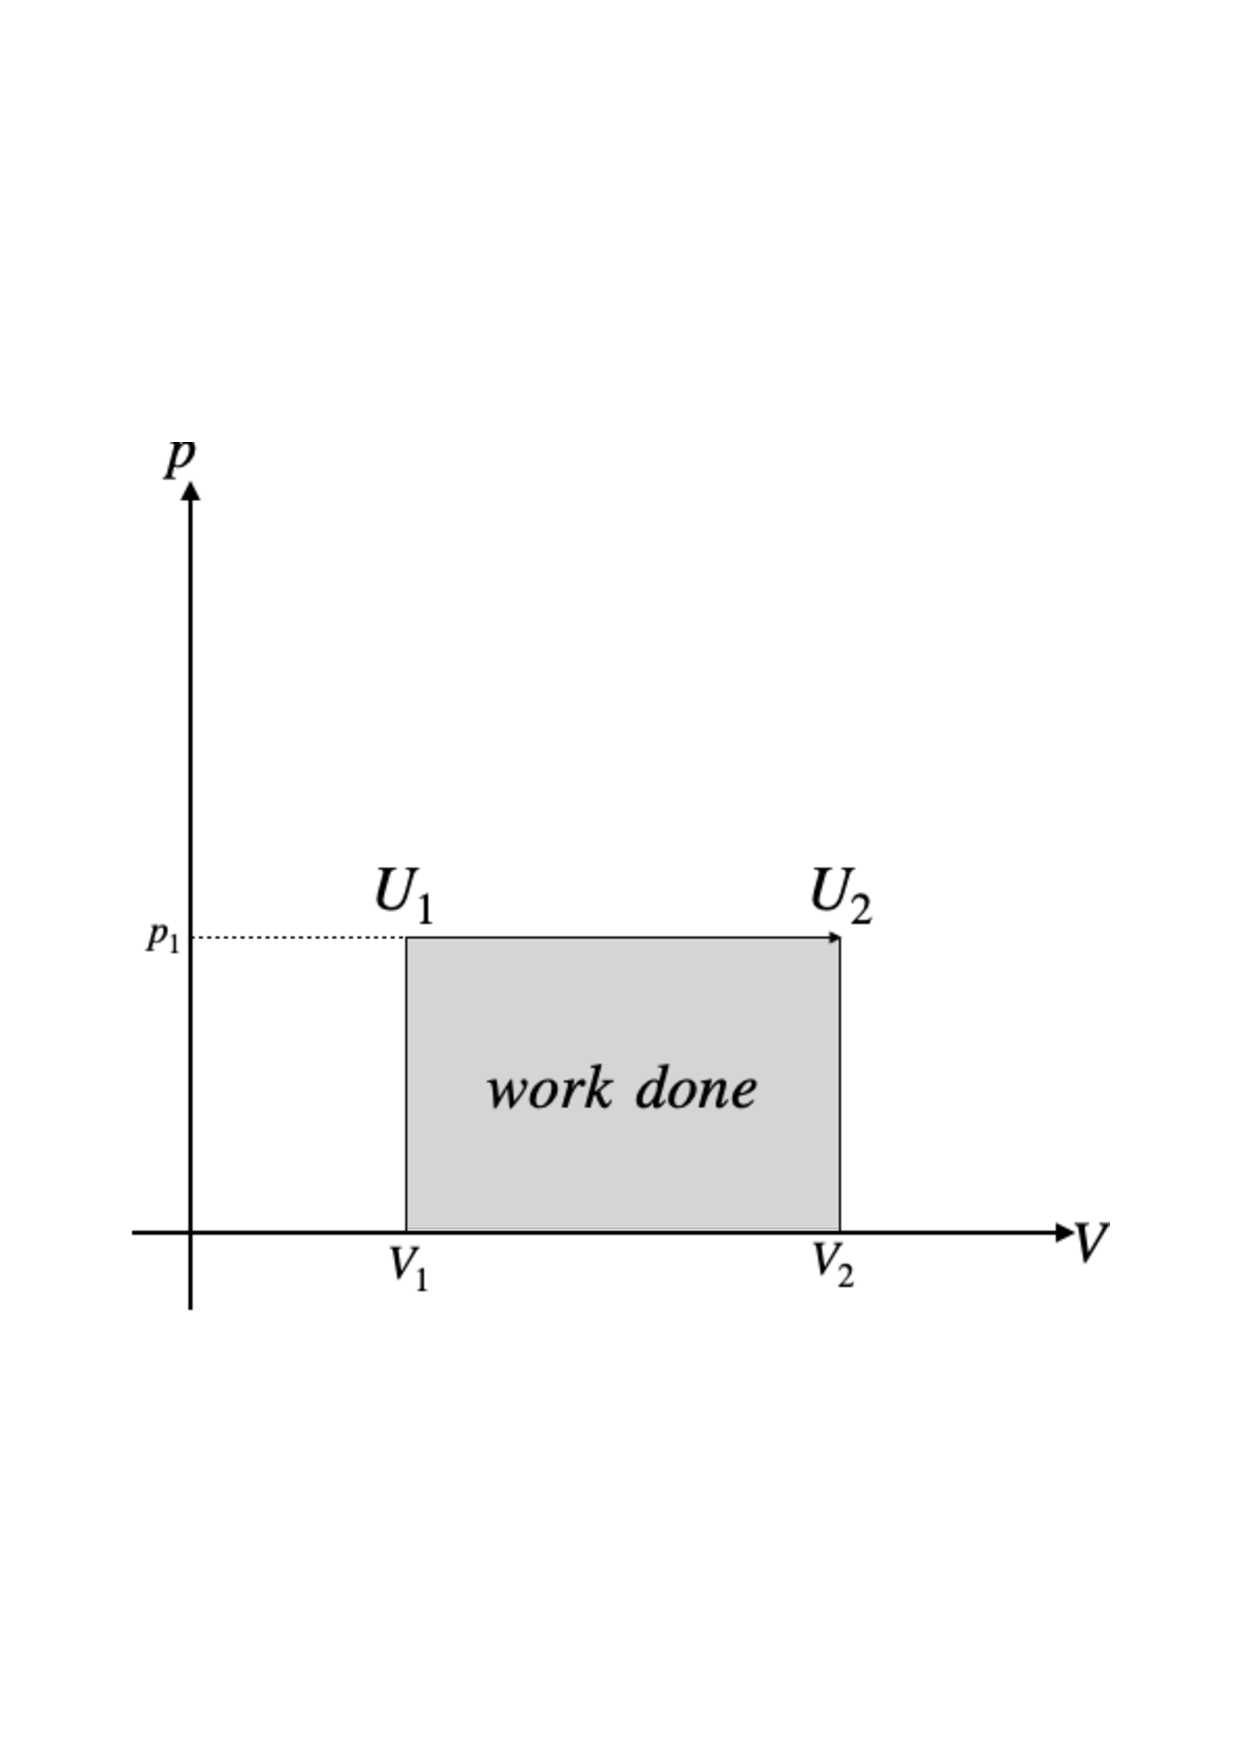
\includegraphics[trim = 50 50 50 50, width=3in]{figures/isobaric_expansion.pdf} 
\end{minipage}	
\begin{minipage}{0.5\textwidth}
   \textbf{Isobaric expansion} \\ \\

   Since volume increases, work done on the gas is negative \\
   Since 
   \[
   T \propto pV
   \]
   Temperature increases, and hence
   \[
   \Delta U > 0
   \]

   Hence heat is transferred into the system
\end{minipage}	

\subsection{Isovolumetric processes}
Pressure changes without a change in volume \\
\begin{minipage}{0.5\textwidth}
      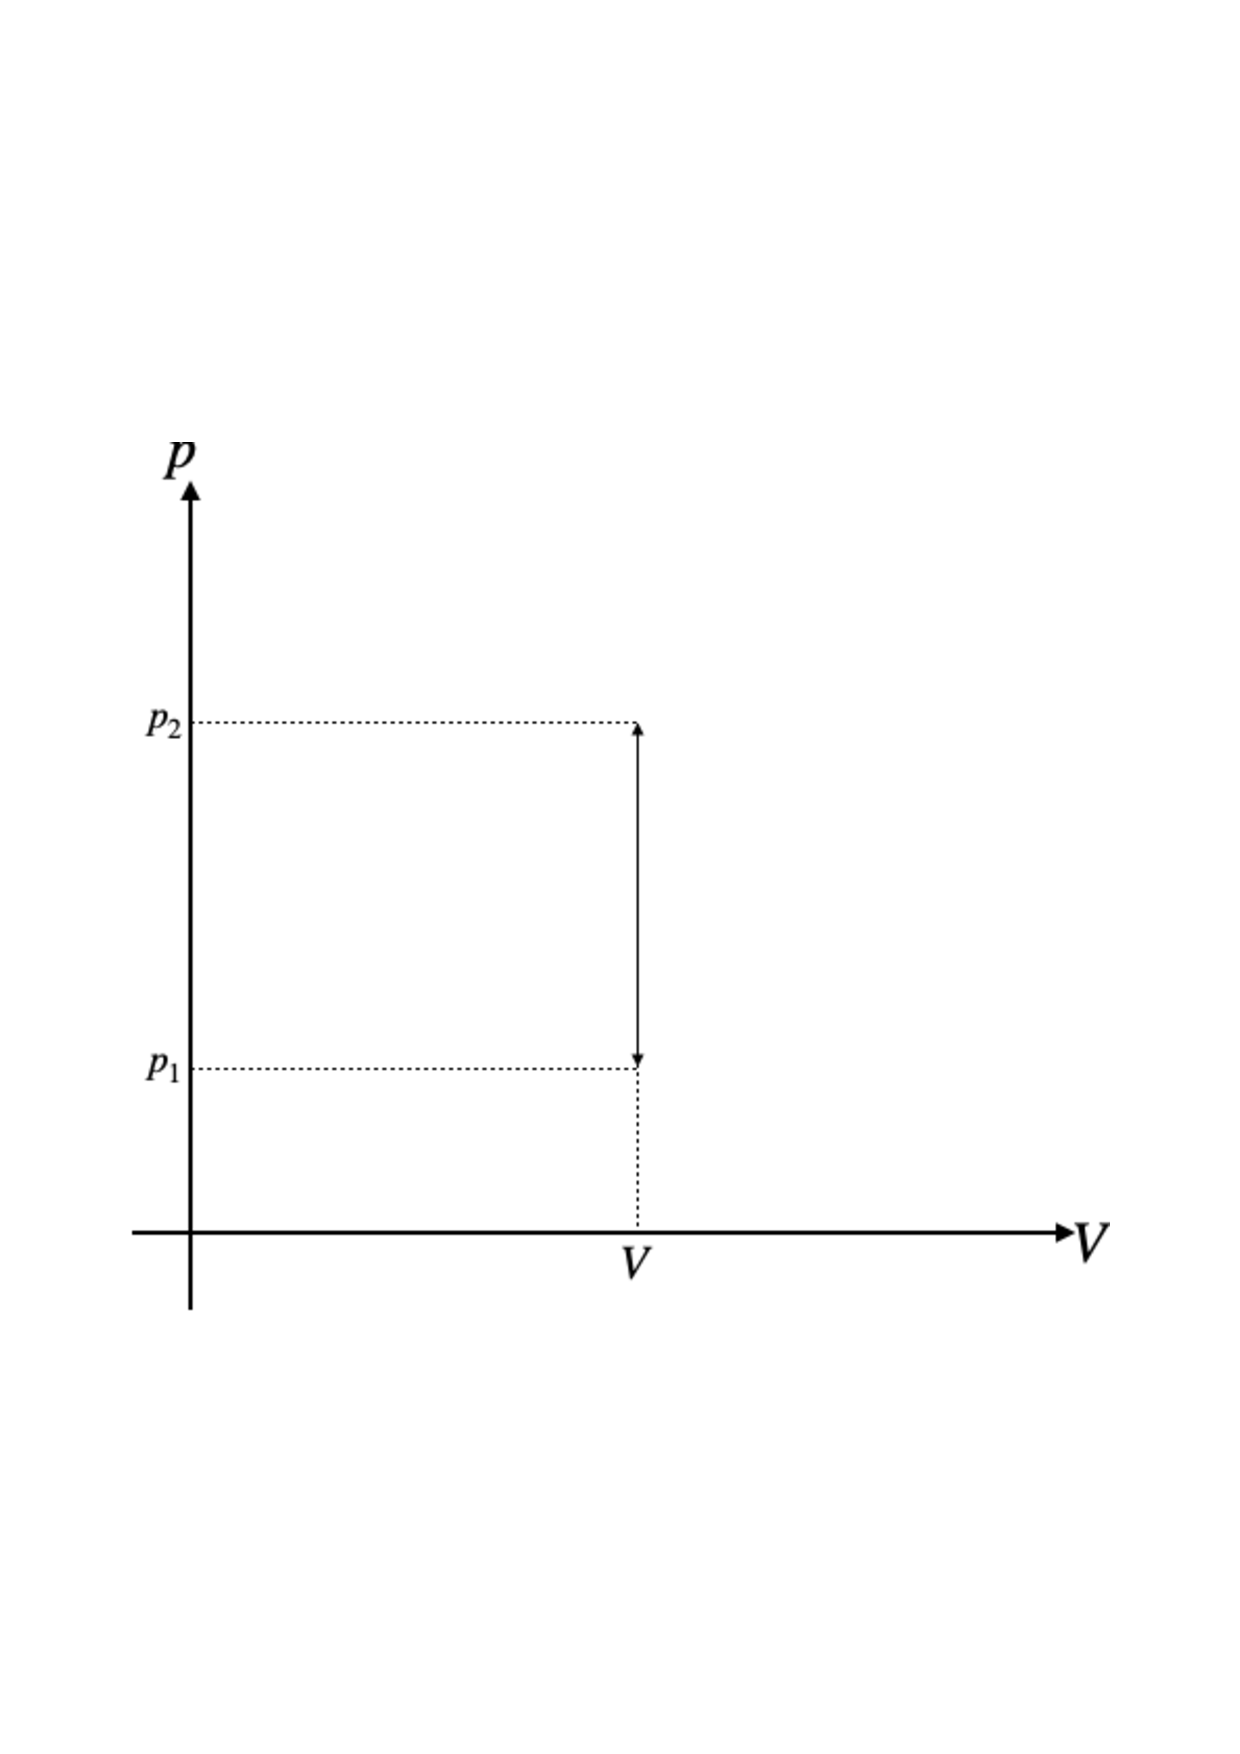
\includegraphics[trim = 50 50 50 50, width=3in]{figures/isovolumetric_process.pdf} 
\end{minipage}	
\begin{minipage}{0.5\textwidth}
   \textbf{Isovolumetric process} \\ \\

   Since $V$ is constant, $W$ = 0
   \[
   \Delta U = Q + 0,\ \Delta U = Q
   \]
   For an increase in pressure, 
   \[
   \Delta U > 0
   \]
   \[
   Q = 0
   \]
\end{minipage}	

\subsection{Isothermal Process}
For a system at constant temperature, and heat exchange happens slowly, such that pressure and volume changes occur without a change in temperature \\

\begin{minipage}{0.5\textwidth}
      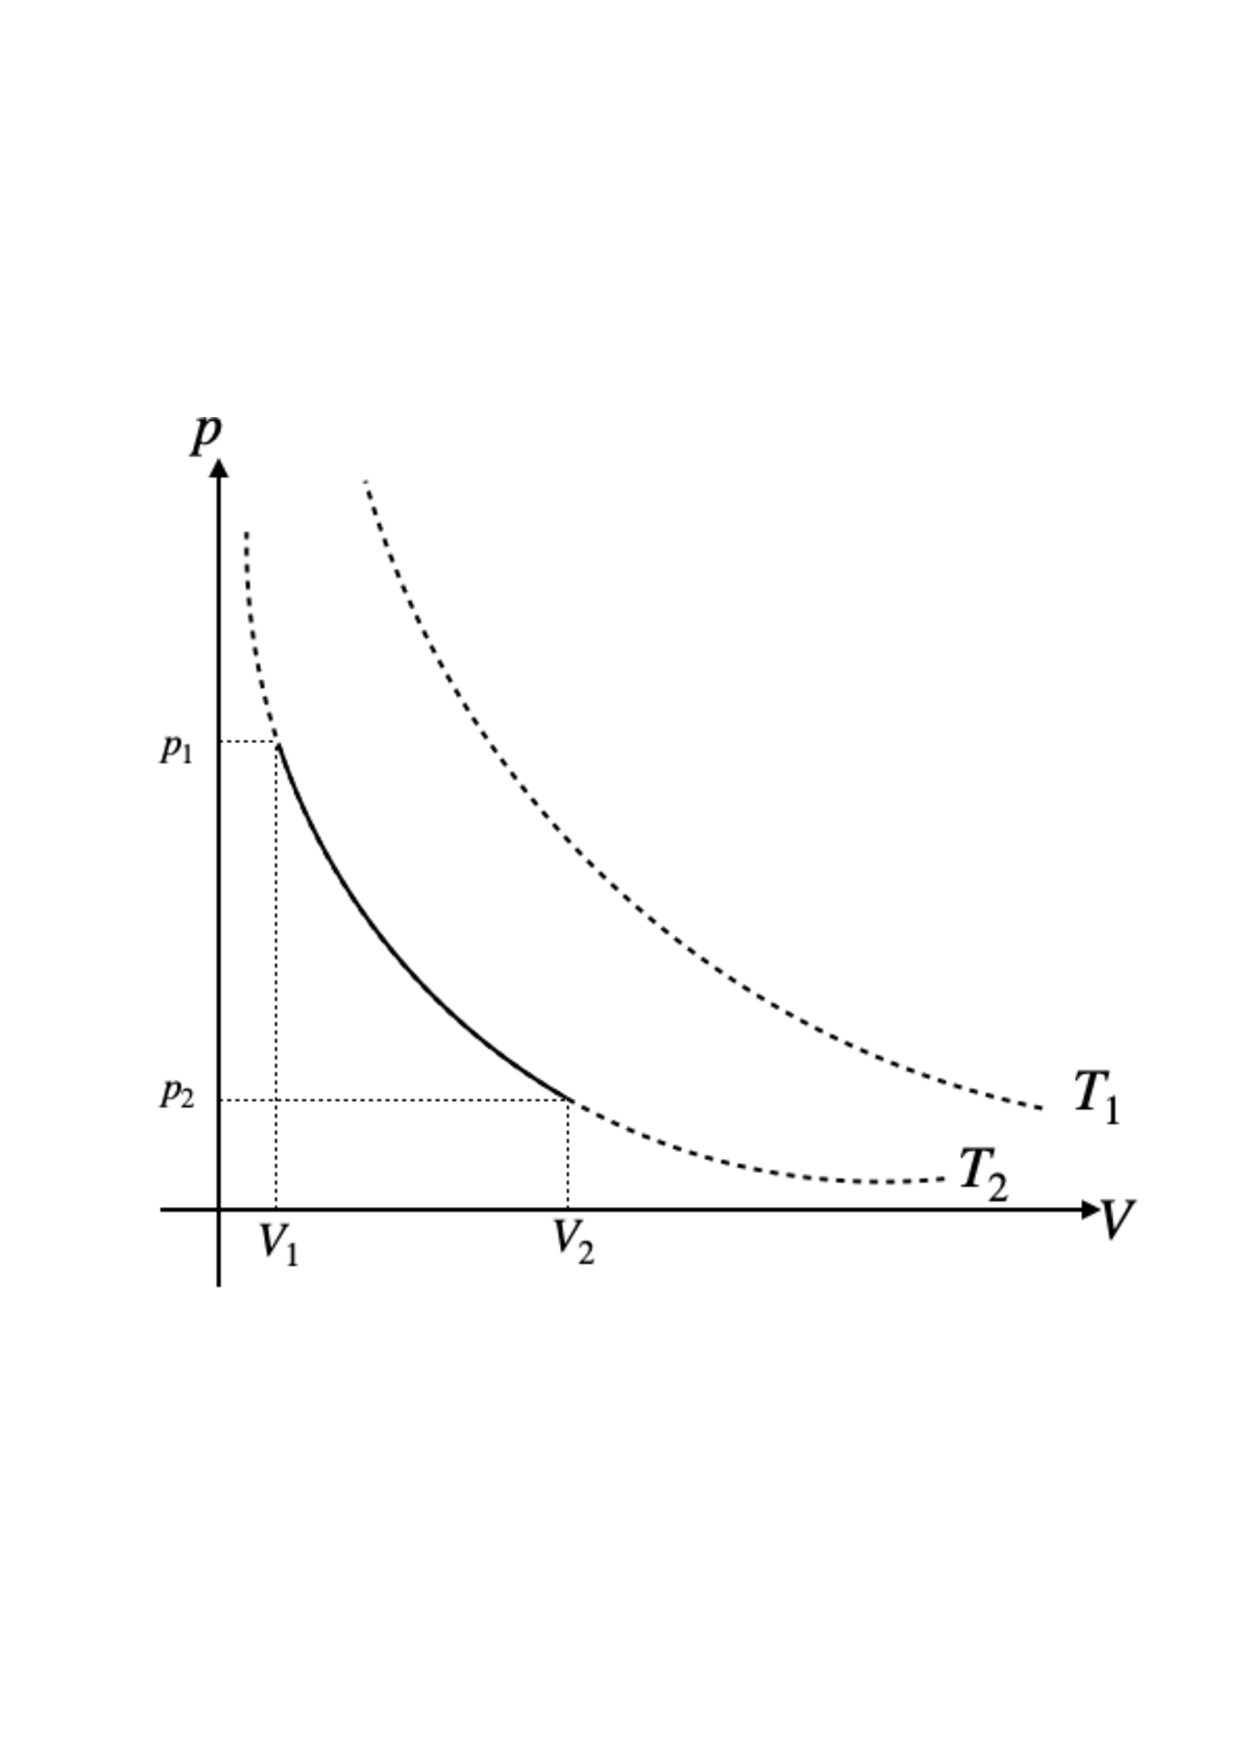
\includegraphics[trim = 50 50 50 50, width=3in]{figures/isothermal_process.pdf} 
\end{minipage}	
\begin{minipage}{0.5\textwidth}
   \textbf{Isothermal expansion} \\ \\

   Along each isotherm, $T$ constant, hence
   \[
   \Delta U = 0
   \]
   \[
   0 = Q + W
   \]
   For an expansion, work is done by the system, hence
   \[
   W < 0, \ hence\ Q > 0
   \]
\end{minipage}	

\subsection{Adiabetic Process}
When a system under goes a change in pressure and volume with no heat being supplied to or lost from the system \\

This could happen if 
\begin{itemize}
   \item system is insulated
   \item the change in pressure and volume happens rapidly and hence no heat exchange with the surrouding occurs
\end{itemize} 
\begin{minipage}{0.5\textwidth}
   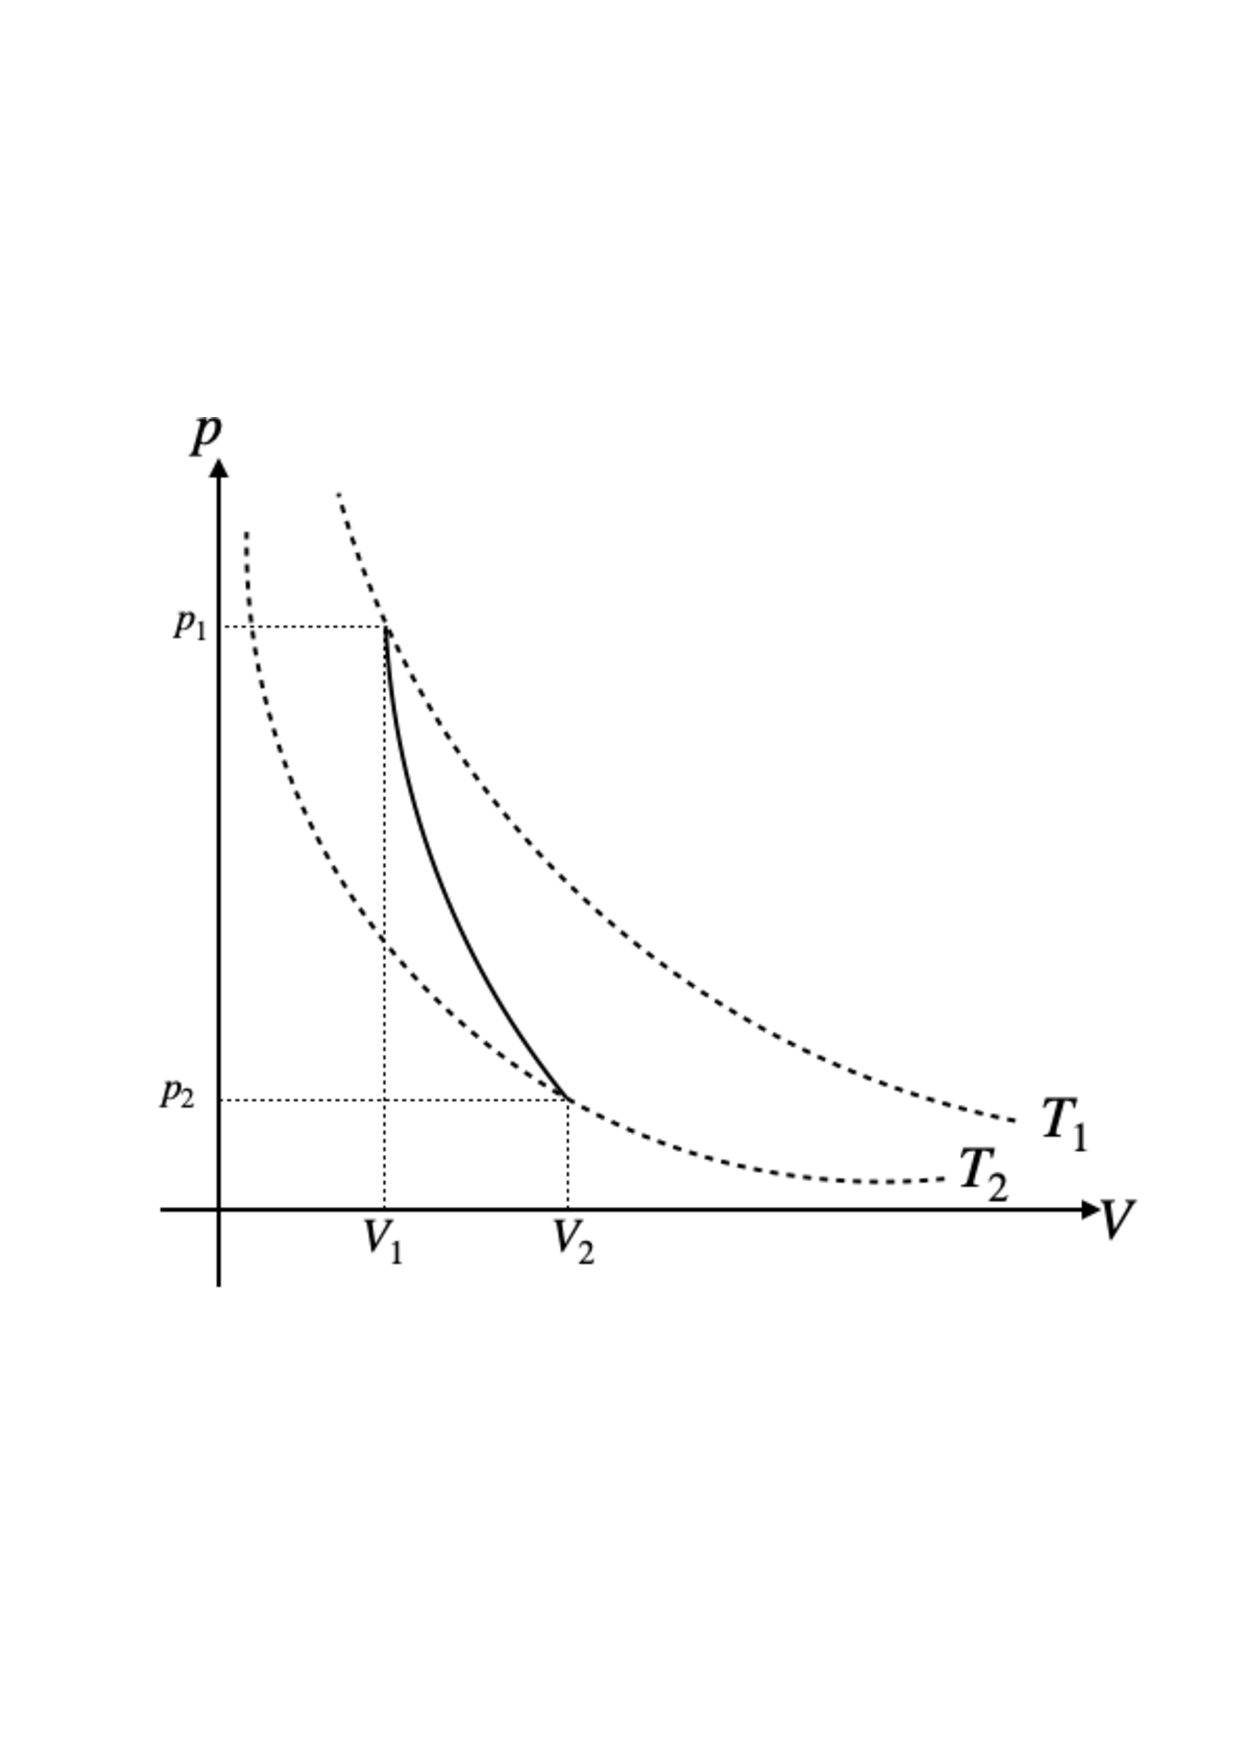
\includegraphics[trim = 50 50 50 50, width=3in]{figures/adiabetic_process.pdf} 
\end{minipage}	
\begin{minipage}{0.5\textwidth}
   For an expansion
   \[
   W < 0
   \]
   pressure decreases, 
   T decreases, hence
   \[
   \Delta U < 0
   \]
\end{minipage}	



\end{document}	
